\section{Vista de Escenarios}
En la siguiente figura, la \ref{fig:Diagrama de Casos de Uso - Vista de Escenarios}, se muestra la vista de escenarios representada por un diagrama de casos de uso. Este diagrama refleja los requerimientos funcionales principales del sistema. Cada caso de uso lo hemos identificado un una nomenclatura CU'X', siendo la letra 'X' el número del caso de uso al que se hace referencia.
\\
\begin{figure}[!h]
	\centering
	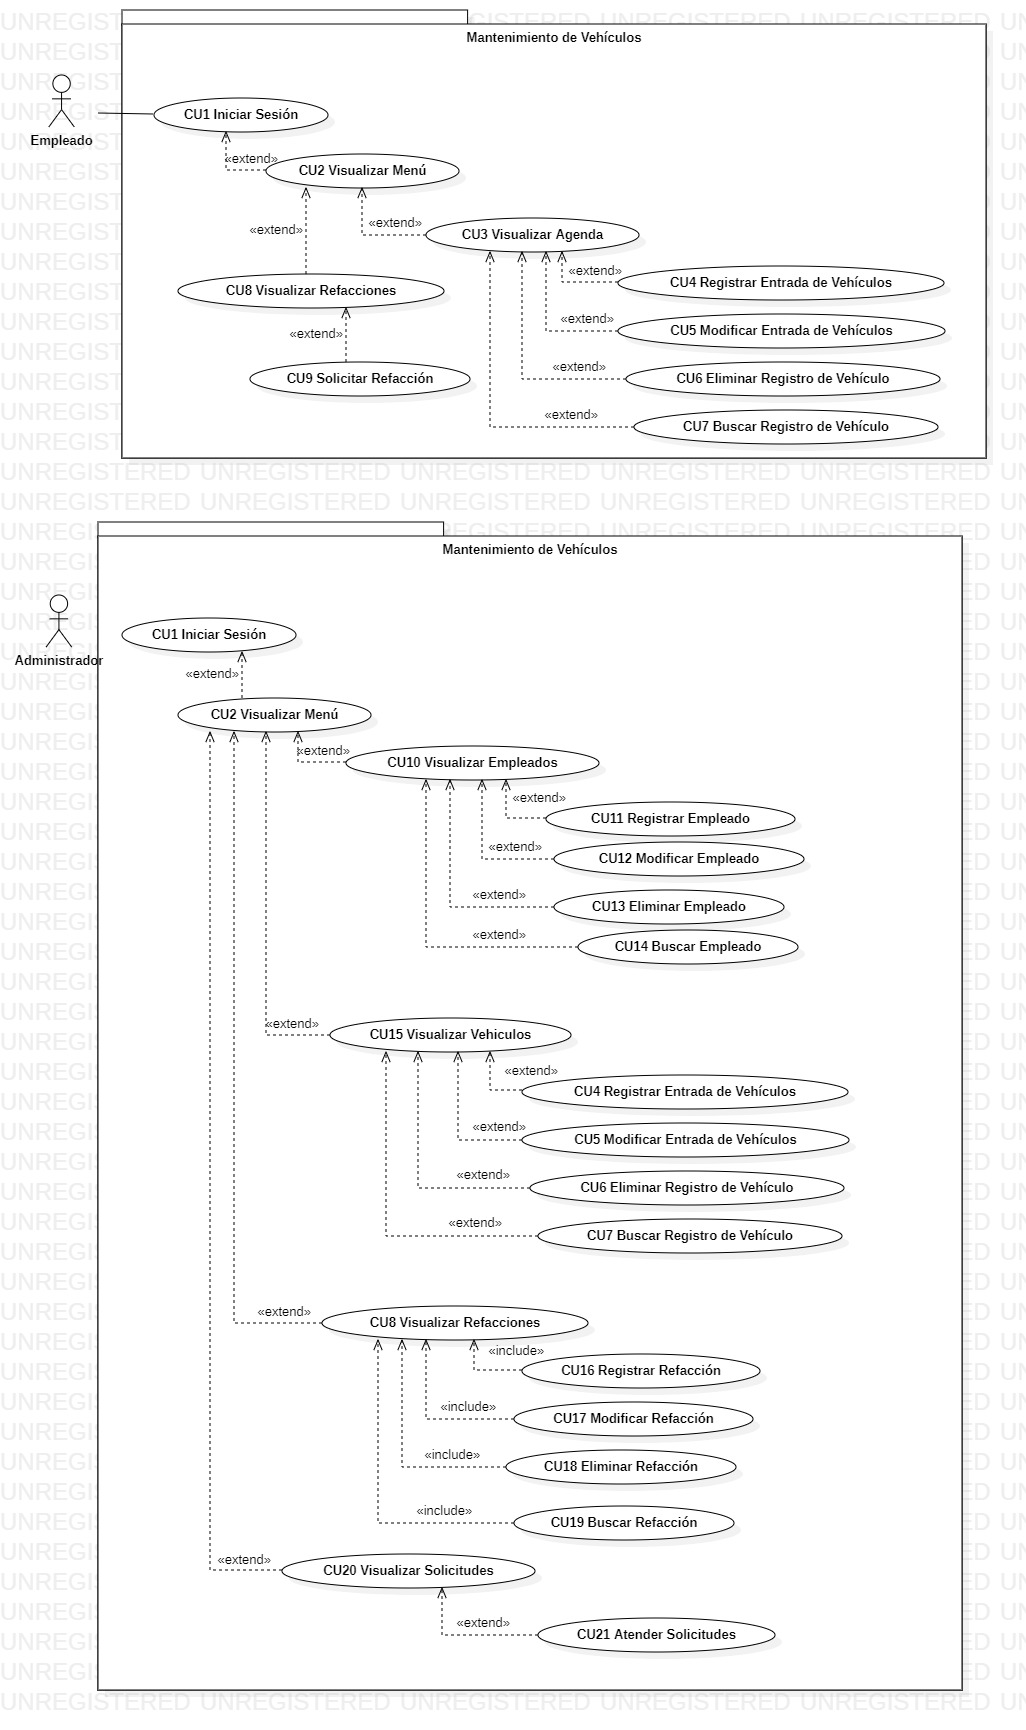
\includegraphics[width=1\textwidth]{./diseno/vescenarios/imagenes/vistaEscenarios}
	\caption{Diagrama de Casos de Uso - Vista de Escenarios}
	\label{fig:Diagrama de Casos de Uso - Vista de Escenarios}
\end{figure}
\\
A continuación se describen a detalle cada uno de los casos de uso que serán implementados en el sistema. Cada uno de estos casos también llevará un diseño de la UI (Interfaz de Usuario) para poder explicar el procedimiento de cada uno de los procesos. Cabe mencionar que estos casos de uso van de la mano con las historias de usuario descritas en el capítulo \ref{chap: historias de usuario}. 

\clearpage

%Contenido de la vista de escenarios
\subsection{CU1 Iniciar Sesión}
Esta pantalla (figura \ref{fig:Pantalla Iniciar Sesion - Vista de Escenarios}) será la primera en aparecer al ejecutarse el sistema. Se compone de un pequeño formulario donde el usuario (Mecánico) deberá teclear sus credenciales otorgadas por la administración de la empresa. Una vez ingresados de manera correcta, deberá pulsar el botón 'Ingresar'.
\\
En caso de que el usuario desee salir del sistema, solo deberá pulsar el botón 'Salir'. 
\\

\begin{figure}[!h]
	\centering
	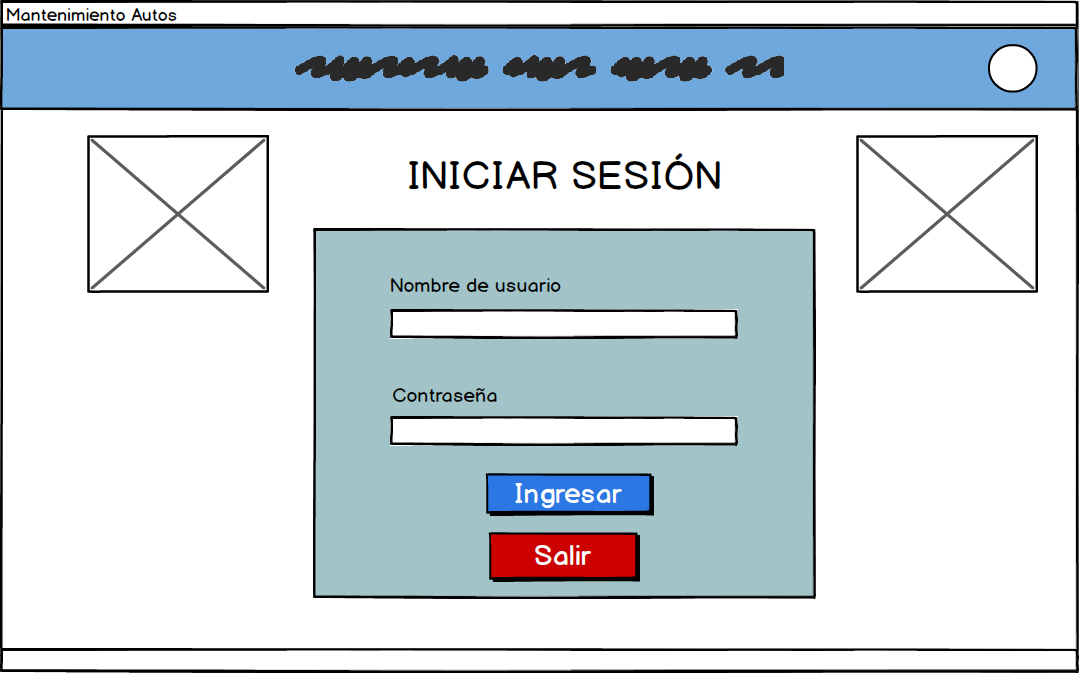
\includegraphics[width=1\textwidth]{./diseno/vescenarios/imagenes/Login}
	\caption{Pantalla Iniciar Sesión - Vista de Escenarios}
	\label{fig:Pantalla Iniciar Sesion - Vista de Escenarios}
\end{figure}
En ese sentido, si el usuario ingresa erróneamente sus credenciales de autenticación, el sistema mostrará un mensaje de alerta (\ref{fig:Alerta1 - Vista de Escenarios}).
\\
\begin{figure}[!h]
	\centering
	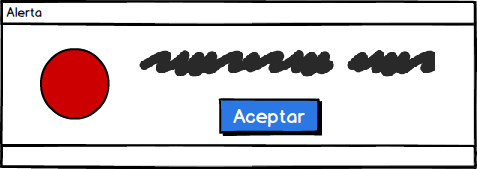
\includegraphics[width=0.5\textwidth]{./diseno/vescenarios/imagenes/alerta}
	\caption{Alerta Datos Erróneos - Vista de Escenarios}
	\label{fig:Alerta1 - Vista de Escenarios}
\end{figure}
\clearpage
\subsection{CU2 Visualizar Menú}
Al momento de ingresar las credenciales y que el sistema otorgue acceso al usuario, aparecerá una pantalla muy simular a la que mostramos a continuación (figura \ref{fig:Pantalla Visualizar Menu - Vista de Escenarios}). Esta pantalla posee el mismo diseño que el inicio de sesión (figura \ref{fig:Pantalla Iniciar Sesion - Vista de Escenarios}), solo que esta vez, se muestran tres opciones principales. 
\begin{itemize}
	\item \textbf{Gestionar Agenda:} En esta opción se desplegará otra pantalla que le dará acceso al usuario a toda la información que desee saber sobre los registros de los vehículos que estén dentro del taller además de la gestión de los mismos.
	\item \textbf{Gestionar Refacciones:} En dado caso que el usuario desee saber sobre la existencia de alguna refacción en particular dentro del almacén del taller además de generar una solicitud para la obtención de una si en necesario.
	\item \textbf{Cancelar:} El usuario desea salir de esa pantalla y regresar a la pantalla de Iniciar Sesión (figura \ref{fig:Pantalla Iniciar Sesion - Vista de Escenarios}).
\end{itemize}
\begin{figure}[!h]
	\centering
	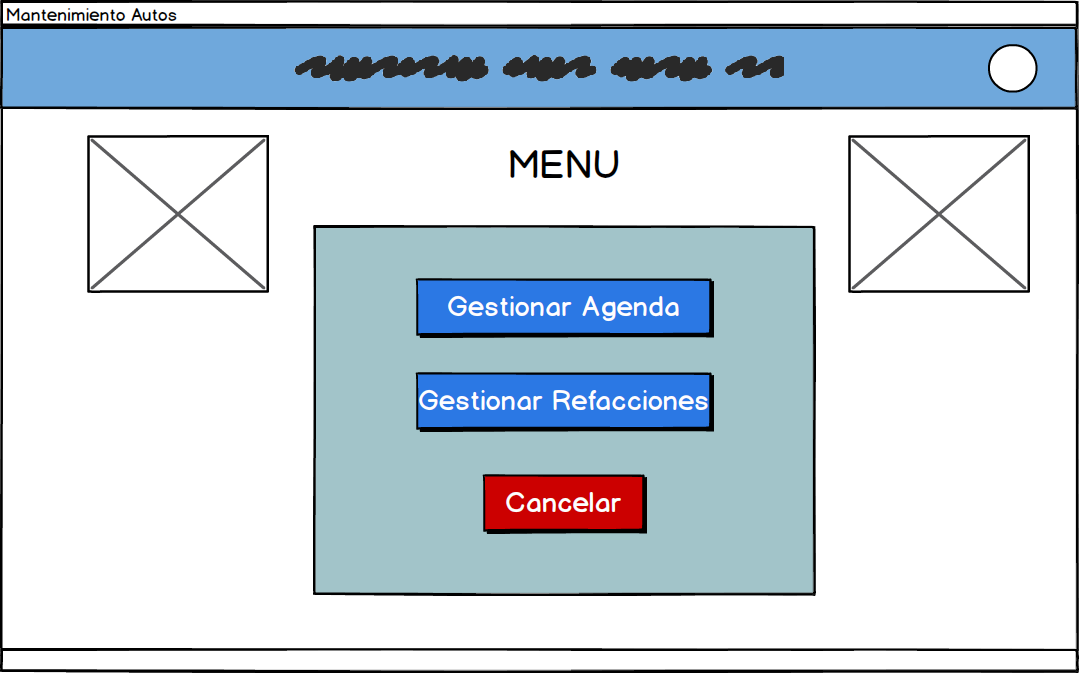
\includegraphics[width=1\textwidth]{./diseno/vescenarios/imagenes/VisualizarMenu}
	\caption{Pantalla Visualizar Menu - Vista de Escenarios}
	\label{fig:Pantalla Visualizar Menu - Vista de Escenarios}
\end{figure}
\clearpage
\subsection{CU3 Visualizar Agenda}
Supongamos que el usuario decide ver todos los registros de los vehículos dentro del taller y elige la opción de Gestionar Agenda, inmediatamente esta pantalla (figura \ref{fig:Pantalla Visualizar Agenda - Vista de Escenarios}) aparecerá. Compuesta principalmente por una tabla donde se mostrarán a manera de lista cada uno de los registros que estén almacenados en la base de datos, en caso de que no exista ningún registro, dicha tabla se mostrará vacía.
\\
En la parte superior derecha hay una barra de búsqueda, se explica a detalle este proceso mas adelante (véase \ref{sub:buscar registro}). 
\\
En la parte inferior se despliegan una serie de botones que permitirán al usuario gestionar esta tabla de registros que se le presentan:
\begin{itemize}
	\item \textbf{Actualizar Registro:} Permite al usuario actualizar la tabla una vez que este haya realizado algún cambio en los registros.
	\item \textbf{Registrar Vehículo:} Despliega una pantalla con un formulario de registro.
	\item \textbf{Modificar Vehículo:} Despliega una pantalla con un formulario de actualización.
	\item \textbf{Eliminar Vehículo:} Despliega una pantalla con un 'mensaje de seguridad'. 
	\item \textbf{Salir:} Regresar al menú de opciones (figura \ref{fig:Pantalla Visualizar Menu - Vista de Escenarios}). 
\end{itemize}
\begin{figure}[!h]
	\centering
	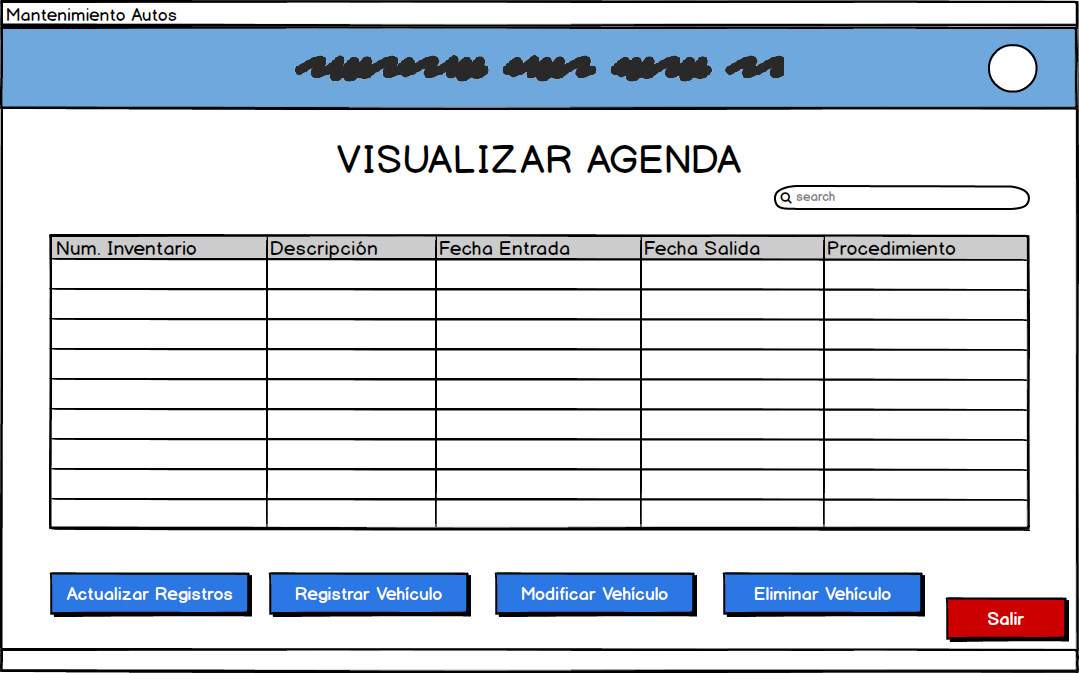
\includegraphics[width=1\textwidth]{./diseno/vescenarios/imagenes/VisualizarAgenda}
	\caption{Pantalla Visualizar Agenda - Vista de Escenarios}
	\label{fig:Pantalla Visualizar Agenda - Vista de Escenarios}
\end{figure}
Cabe señalar que el usuario debe de elegir un registro en la tabla para poder realizar alguna de las acciones antes mencionadas, de lo contrario aparecerá un 'mensaje de alerta' (figura \ref{fig:Alerta - Vista de Escenarios}) donde le de a entender al usuario lo que debe de hacer antes de relizar cualquier acción sobre algún registro.
\begin{figure}[!h]
	\centering
	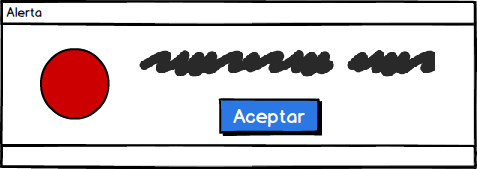
\includegraphics[width=0.5\textwidth]{./diseno/vescenarios/imagenes/alerta}
	\caption{Alerta Elección de Registro - Vista de Escenarios}
	\label{fig:Alerta - Vista de Escenarios}
\end{figure}
\clearpage
\subsection{CU4 Registrar Entrada de Vehículo}
Pantalla que aparece al presionar el botón de 'Registrar Vehículo' en la visualización de agenda (figura \ref{fig:Pantalla Visualizar Menu - Vista de Escenarios}). Este formulario le solicita al usuario los siguientes campos: Número de Inventario, Descripción, Fecha de Entrada, Fecha de Salida y el Procedimiento que se le hará al vehículo. 
\\
Cuenta con dos botones en la parte inferior, uno para proceder a enviar el registro a la base de datos y otro para cancelar en caso de que el usuario así lo desee. 
\\
\begin{figure}[!h]
	\centering
	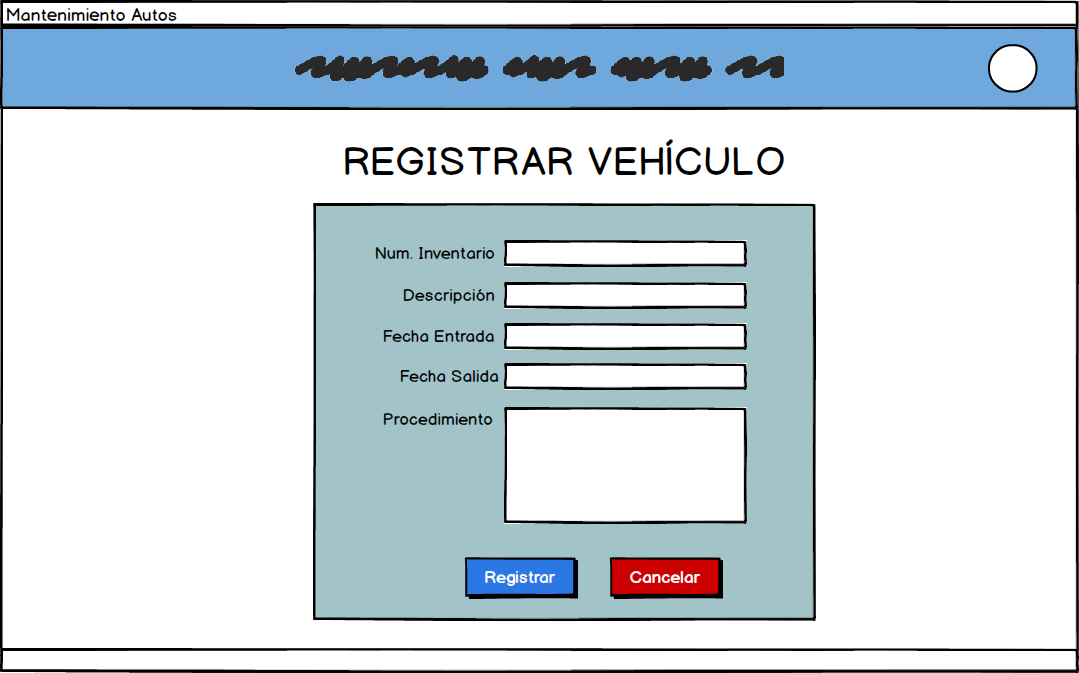
\includegraphics[width=0.9\textwidth]{./diseno/vescenarios/imagenes/registrarVehiculo}
	\caption{Pantalla Registrar Vehículo - Vista de Escenarios}
	\label{fig:Pantalla Registrar Vehículo - Vista de Escenarios}
\end{figure}
\\
En caso de que el usuario ingrese algún dato mal, es decir, que los campos no estén llenos o el formato de la información no es el correcto, aparecerá una alerta como la que se muestra a continuación (figura \ref{fig:Alerta2 - Vista de Escenarios}):
\begin{figure}[!h]
	\centering
	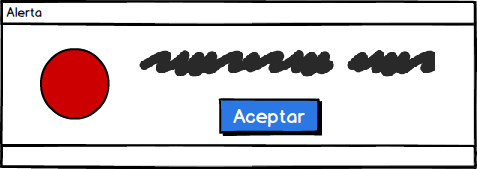
\includegraphics[width=0.4\textwidth]{./diseno/vescenarios/imagenes/alerta}
	\caption{Alerta Confirmación de Registro - Vista de Escenarios}
	\label{fig:Alerta2 - Vista de Escenarios}
\end{figure}
\clearpage
\subsection{CU5 Modificar Registro de Vehículo}
Esta pantalla es muy similar a la del 'Registro de Vehículo' (figura \ref{fig:Pantalla Registrar Vehículo - Vista de Escenarios}), solo que esta vez cuando el usuario desee modificar un registro en específico este formulario aparecerá con todos los campos llenos para que el usuario pueda modificar el que necesite. 
\\
En la parte inferior de la pantalla hay dos botones; el primero de ellos, el botón 'Modificar' lleva la información a la base de datos. El segundo, botón 'Cancelar' cierra esta pantalla y no hay alteración en los datos. 
\begin{figure}[!h]
	\centering
	\includegraphics[width=1\textwidth]{./diseno/vescenarios/imagenes/modificarVehículo}
	\caption{Pantalla Modificar Registro de Vehículo - Vista de Escenarios}
	\label{fig:Pantalla Modificar Registro de Vehículo - Vista de Escenarios}
\end{figure}
\\
En caso de que el usuario actualice algún dato mal, es decir, que los campos no estén llenos o el formato de la información no es el correcto, aparecerá una alerta como la que se muestra a continuación (figura \ref{fig:Alerta3 - Vista de Escenarios}):
\begin{figure}[!h]
	\centering
	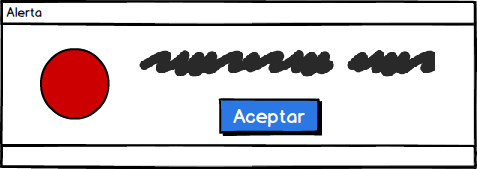
\includegraphics[width=0.5\textwidth]{./diseno/vescenarios/imagenes/alerta}
	\caption{Alerta Modificación - Vista de Escenarios}
	\label{fig:Alerta3 - Vista de Escenarios}
\end{figure}
\clearpage
\subsection{CU6 Eliminar Registro de Vehículo}
Esta pantalla es muy similar a la de Registrar Vehículo (figura \ref{fig:Pantalla Registrar Vehículo - Vista de Escenarios}) y a la de Modificar Vehículo (figura \ref{fig:Pantalla Modificar Registro de Vehículo - Vista de Escenarios}), sin embargo, esta pantalla esta diseñada para ser un 'mensaje de seguridad'. Muestra los datos que el usuario desea eliminar y al pulsar el botón 'Aceptar', el sistema ordena a la base de datos eliminar ese registro. Por otro lado, el botón 'Cancelar', cierra ese mensaje de seguridad y volvemos a la pantalla de Visualizar Agenda (figura \ref{fig:Pantalla Visualizar Agenda - Vista de Escenarios}).
\\
\begin{figure}[!h]
	\centering
	\includegraphics[width=1\textwidth]{./diseno/vescenarios/imagenes/eliminarVehículo}
	\caption{Pantalla Eliminar Registro de Vehículo - Vista de Escenarios}
	\label{fig:Pantalla Eliminar Registro de Vehículo - Vista de Escenarios}
\end{figure}
\\
Cuando se ha eliminado el registro de manera exitosa en la base de datos, el sistema mostrará una alerta (figura \ref{fig:Alerta4 - Vista de Escenarios}) como confirmación de que se ha borrado el registro de la base de datos.
\begin{figure}[!h]
	\centering
	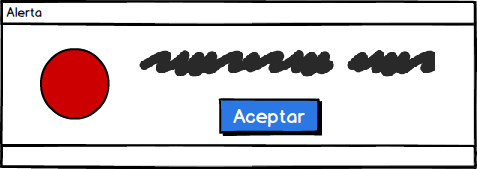
\includegraphics[width=0.5\textwidth]{./diseno/vescenarios/imagenes/alerta}
	\caption{Alerta Confirmación de Eliminación- Vista de Escenarios}
	\label{fig:Alerta4 - Vista de Escenarios}
\end{figure}
\subsection{CU7 Buscar Registro de Vehículo \label{sub:buscar registro}}
En este proceso no existe una pantalla como tal simplemente en la Visualización de la Agenda (figura \ref{fig:Pantalla Visualizar Agenda (busqueda)- Vista de Escenarios}) hay una barra de búsqueda en la parte superior donde el usuario podrá teclear el Número de Inventario del vehículo que desee. Si existe ese registro dentro de la base de datos, el sistema lo mostrará en la tabla. Caso contrario, si no existe, mostrará la tabla vacía. 
\begin{figure}[!h]
	\centering
	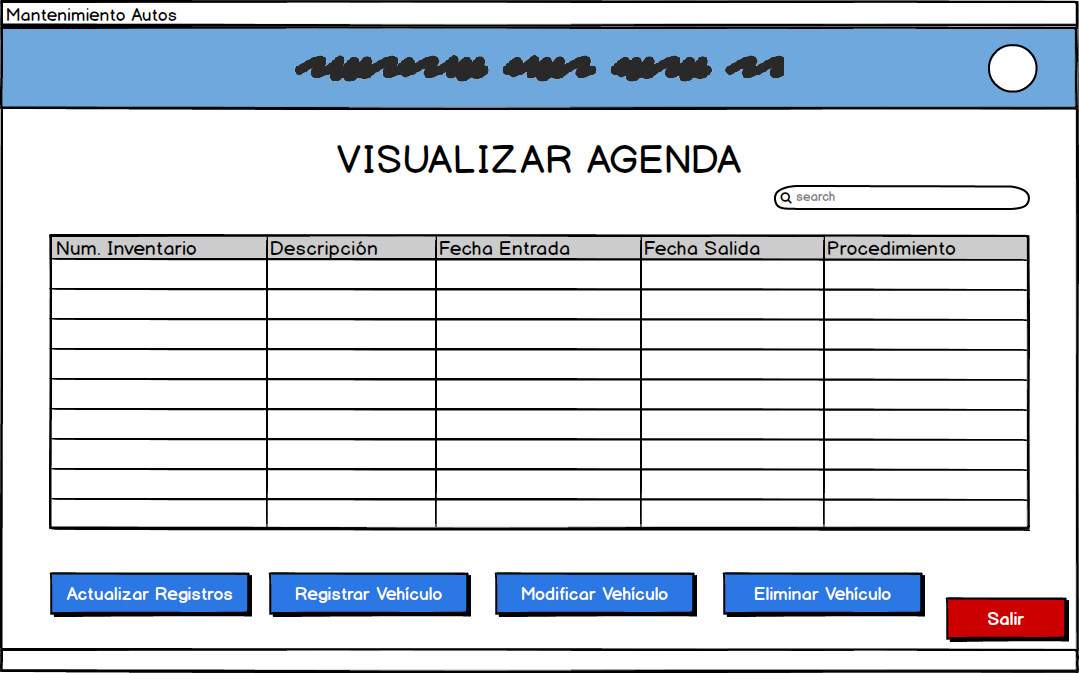
\includegraphics[width=1\textwidth]{./diseno/vescenarios/imagenes/VisualizarAgenda}
	\caption{Pantalla Visualizar Agenda (Búsqueda) - Vista de Escenarios}
	\label{fig:Pantalla Visualizar Agenda (busqueda)- Vista de Escenarios}
\end{figure}
\clearpage
\subsection{CU8 Visualizar Refacciones Disponibles}
Regresando un poco a la pantalla de Visualización del Menú (figura \ref{fig:Pantalla Visualizar Menu - Vista de Escenarios}), al pulsar el botón de 'Gestionar las Refacciones', aparece esta pantalla. Muy simular a la visualización de los registros pero aquí el usuario solamente podrá ver y buscar las refacciones que hay en existencia en el almacén del taller. En caso de que no exista alguno, podrá presionar el botón de la parte inferior 'Solicitar Refacción'.
\\
En la tabla el usuario podrá observar los registros a manera de lista dentro de una tabla, con los campos: Num. de Solicitud, una Descripción, la Fecha de Solicitud y la Existencia en almacén. 
\\
Al presionar el botón de salir, el sistema cerrará esta pantalla y regresará a la Visualización del Menú. 
\begin{figure}[!h]
	\centering
	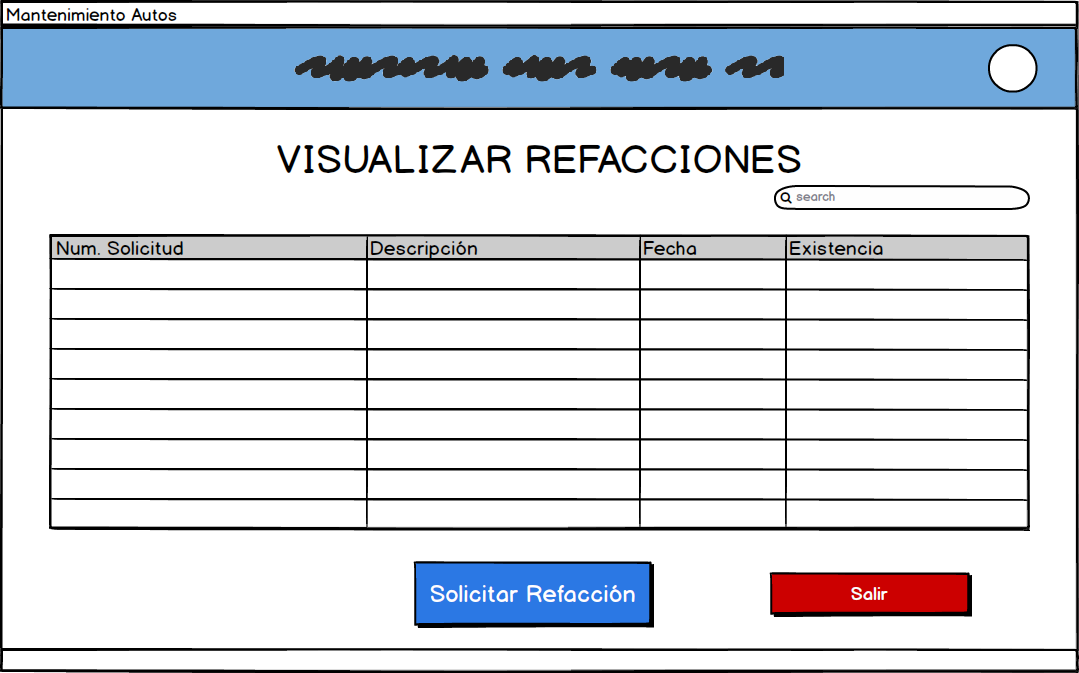
\includegraphics[width=1\textwidth]{./diseno/vescenarios/imagenes/VisualizarRefacciones}
	\caption{Pantalla Visualizar Refacciones - Vista de Escenarios}
	\label{fig:Pantalla Visualizar Refaccioes - Vista de Escenarios}
\end{figure}
\clearpage
\subsection{CU9 Solicitar Refacción}
Al entrar a esta parte del sistema, se despliega esta pantalla. Es un formulario de registro para la solicitud de alguna pieza en especifico. Solicitará un identificador (en este caso manejamos un Número de Solicitud), la Fecha en que se solicita y una Descripción donde se podrá agregar alguna otra información como el nombre o modelo. 
\\
Un vez llenado el formulario el usuario podrá pulsar el botón de 'Solicitar' para registrar esto en la base de datos. En caso de que el usuario desee salir de esta pantalla, simplemente deberá pulsar el botón 'Cancelar'.
\begin{figure}[!h]
	\centering
	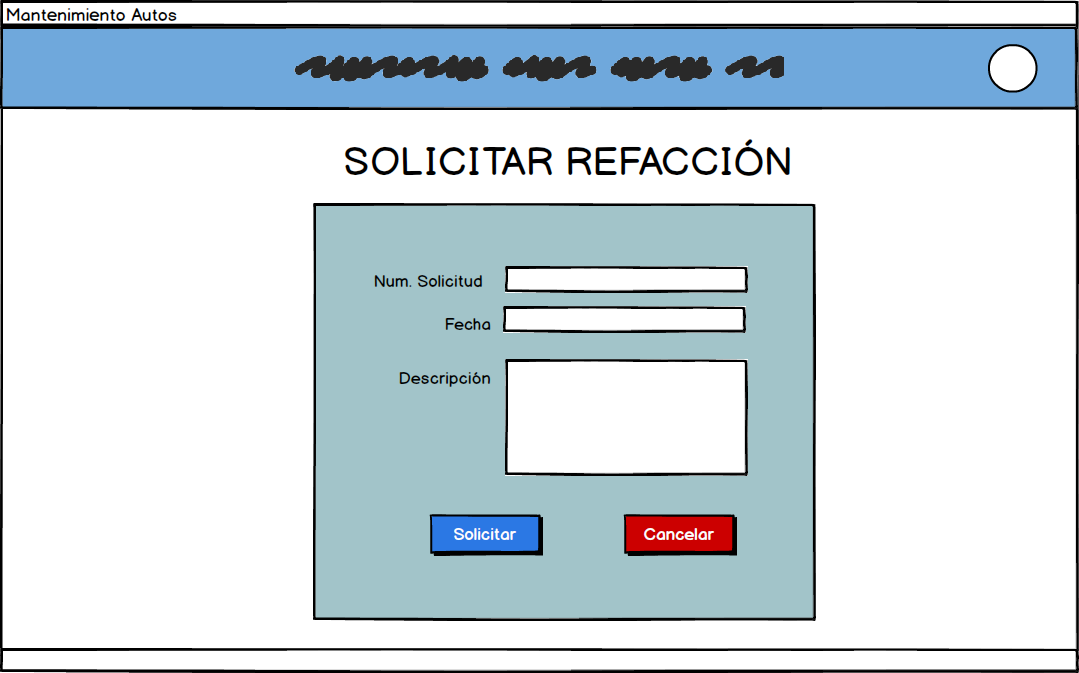
\includegraphics[width=1\textwidth]{./diseno/vescenarios/imagenes/solicitarRefaccion}
	\caption{Pantalla Solicitar Refacción - Vista de Escenarios}
	\label{fig:Pantalla Solicitar Refaccion - Vista de Escenarios}
\end{figure}
En caso de que el usuario ingrese de manera incorrecta alguno de los campos, el sistema mostrará un 'mensaje de alerta' (figura \ref{fig:Alerta5 - Vista de Escenarios}) informado del error que ha cometido. 
\begin{figure}[!h]
	\centering
	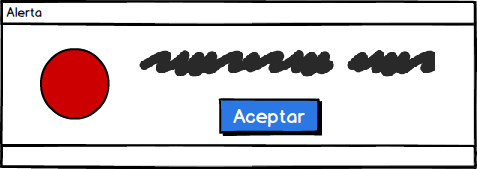
\includegraphics[width=0.4\textwidth]{./diseno/vescenarios/imagenes/alerta}
	\caption{Alerta Confirmación de Registro - Vista de Escenarios}
	\label{fig:Alerta5 - Vista de Escenarios}
\end{figure}
